\documentclass[11pt]{scrartcl} % Font size

%%%%%%%%%%%%%%%%%%%%%%%%%%%%%%%%%%%%%%%%%
% Wenneker Assignment
% Structure Specification File
% Version 2.0 (12/1/2019)
%
% This template originates from:
% http://www.LaTeXTemplates.com
%
% Authors:
% Vel (vel@LaTeXTemplates.com)
% Frits Wenneker
%
% License:
% CC BY-NC-SA 3.0 (http://creativecommons.org/licenses/by-nc-sa/3.0/)
%
%%%%%%%%%%%%%%%%%%%%%%%%%%%%%%%%%%%%%%%%%

%----------------------------------------------------------------------------------------
%	PACKAGES AND OTHER DOCUMENT CONFIGURATIONS
%----------------------------------------------------------------------------------------

\usepackage{amsmath, amsfonts, amsthm} % Math packages

\usepackage{listings} % Code listings, with syntax highlighting

\usepackage[english]{babel} % English language hyphenation

\usepackage[xetex]{graphicx}
%\usepackage{graphicx} % Required for inserting images
\graphicspath{{Figures/}{./}} % Specifies where to look for included images (trailing slash required)

\usepackage{booktabs} % Required for better horizontal rules in tables

\numberwithin{equation}{section} % Number equations within sections (i.e. 1.1, 1.2, 2.1, 2.2 instead of 1, 2, 3, 4)
\numberwithin{figure}{section} % Number figures within sections (i.e. 1.1, 1.2, 2.1, 2.2 instead of 1, 2, 3, 4)
\numberwithin{table}{section} % Number tables within sections (i.e. 1.1, 1.2, 2.1, 2.2 instead of 1, 2, 3, 4)

\setlength\parindent{0pt} % Removes all indentation from paragraphs

\usepackage{enumitem} % Required for list customisation
\setlist{noitemsep} % No spacing between list items

%----------------------------------------------------------------------------------------
%	DOCUMENT MARGINS
%----------------------------------------------------------------------------------------

\usepackage{geometry} % Required for adjusting page dimensions and margins

\geometry{
	paper=a4paper, % Paper size, change to letterpaper for US letter size
	top=2.5cm, % Top margin
	bottom=3cm, % Bottom margin
	left=3cm, % Left margin
	right=3cm, % Right margin
	headheight=0.75cm, % Header height
	footskip=1.5cm, % Space from the bottom margin to the baseline of the footer
	headsep=0.75cm, % Space from the top margin to the baseline of the header
	%showframe, % Uncomment to show how the type block is set on the page
}

%----------------------------------------------------------------------------------------
%	FONTS
%----------------------------------------------------------------------------------------

\usepackage[utf8]{inputenc} % Required for inputting international characters
\usepackage[T1]{fontenc} % Use 8-bit encoding

\usepackage{fourier} % Use the Adobe Utopia font for the document

%----------------------------------------------------------------------------------------
%	SECTION TITLES
%----------------------------------------------------------------------------------------

\usepackage{sectsty} % Allows customising section commands

\sectionfont{\vspace{6pt}\centering\normalfont\scshape} % \section{} styling
\subsectionfont{\normalfont\bfseries} % \subsection{} styling
\subsubsectionfont{\normalfont\itshape} % \subsubsection{} styling
\paragraphfont{\normalfont\scshape} % \paragraph{} styling

%----------------------------------------------------------------------------------------
%	HEADERS AND FOOTERS
%----------------------------------------------------------------------------------------

\usepackage{scrlayer-scrpage} % Required for customising headers and footers

\ohead*{} % Right header
\ihead*{} % Left header
\chead*{} % Centre header

\ofoot*{} % Right footer
\ifoot*{} % Left footer
\cfoot*{\pagemark} % Centre footer
 % Include the file specifying the document structure and custom commands
% LaTeX settings for MATLAB code listings
% based on Ted Pavlic's settings in http://links.tedpavlic.com/ascii/homework_new_tex.ascii
\usepackage{listings}
\usepackage[usenames,dvipsnames]{color}

% This is the color used for MATLAB comments below
\definecolor{MyDarkGreen}{rgb}{0.0,0.4,0.0}

% For faster processing, load Matlab syntax for listings
\lstloadlanguages{Matlab}%
\lstset{language=Matlab,                        % Use MATLAB
        frame=single,                           % Single frame around code
        basicstyle=\scriptsize\ttfamily,             % Use small true type font
        keywordstyle=[1]\color{Blue}\bfseries,        % MATLAB functions bold and blue
        keywordstyle=[2]\color{Purple},         % MATLAB function arguments purple
        keywordstyle=[3]\color{Blue}\underbar,  % User functions underlined and blue
        identifierstyle=,                       % Nothing special about identifiers
                                                % Comments small dark green courier
        commentstyle=\usefont{T1}{pcr}{m}{sl}\color{MyDarkGreen}\small,
        stringstyle=\color{Purple},             % Strings are purple
        showstringspaces=false,                 % Don't put marks in string spaces
        tabsize=3,                              % 5 spaces per tab
        %
        %%% Put standard MATLAB functions not included in the default
        %%% language here
        morekeywords={xlim,ylim,var,alpha,factorial,poissrnd,normpdf,normcdf,imresize,double,immse,fspecial,cell2mat,circshift,cell},
        %
        %%% Put MATLAB function parameters here
        morekeywords=[2]{on, off, interp},
        %
        %%% Put user defined functions here
        morekeywords=[3]{FindESS, homework_example},
        %
        morecomment=[l][\color{Blue}]{...},     % Line continuation (...) like blue comment
        numbers=left,                           % Line numbers on left
        firstnumber=1,                          % Line numbers start with line 1
        numberstyle=\tiny\color{Blue},          % Line numbers are blue
        stepnumber=1                            % Line numbers go in steps of 5
        }

% Includes a MATLAB script.
% The first parameter is the label, which also is the name of the script
%   without the .m.
% The second parameter is the optional caption.
\newcommand{\matlabscript}[2]
  {\begin{itemize}\item[]\lstinputlisting[caption=#2,label=#1]{#1.m}\end{itemize}}


\usepackage{fontspec}
\setmainfont{Tinos Nerd Font} %nice font for english and greek

\usepackage{hyperref} %for hyperlinks
\hypersetup{
    colorlinks=true,
    linkcolor=blue,
    filecolor=magenta,
    urlcolor=cyan,
}
%----------------------------------------------------------------------------------------
%	TITLE SECTION
%----------------------------------------------------------------------------------------

\title{
	\normalfont\normalsize
	\textsc{Technical University of Crete, ECE}\\ % Your university, school and/or department name(s)
	\vspace{25pt} % Whitespace
	\rule{\linewidth}{0.5pt}\\ % Thin top horizontal rule
	\vspace{20pt} % Whitespace
	{\Huge Digital Image Processing}\\ % The assignment title

	{\huge Eighth Lab Report}\\ % The assignment title
	\vspace{12pt} % Whitespace
	\rule{\linewidth}{2pt}\\ % Thick bottom horizontal rule
	\vspace{12pt} % Whitespace
}

\author{\LARGE{Τσιαούσης Χρήστος}\\
		\texttt{2016030017}
		\and
		\LARGE{Πρωτοπαπαδάκης Γιώργος}\\
		\texttt{2016030134}}% Your name

\date{\normalsize\today} % Today's date (\today) or a custom date

\begin{document}

\maketitle % Print the title

\section{Σκοπός Εργαστηρίου}

\begin{figure}[h]
    \centering
    \makebox[\textwidth]{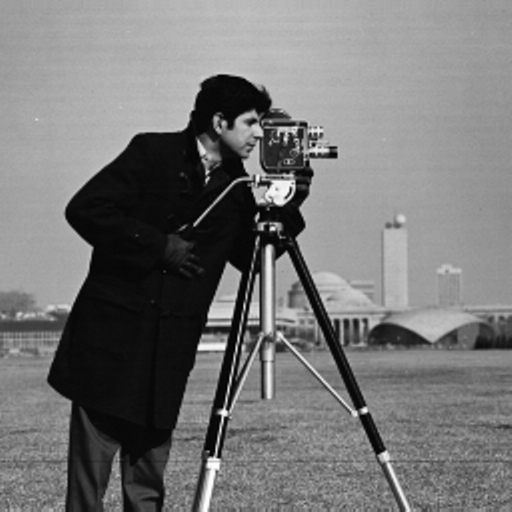
\includegraphics[width=0.4\paperwidth]{cameraman.jpg}}
    \caption{Original Image.}
\end{figure}

\textit{Ο Κώδικας βρίσκεται και συγκεντρωτικά στο τελευταίο κεφάλαιο}

\clearpage
Σκοπός του εργαστηρίου είναι η κατανόηση όλων, πλέον, των μεθόδων συνέλιξης
στις δύο διαστάσεις.

\section{Υλοποίηση}
\subsection*{Βήματα 1-2}
Trivial...
\matlabscript{1}{Βήματα 1-2}

\subsection*{Βήματα 3-4}
Το βήμα αυτό υλοποιήθηκε με τις έτοιμες συναρτήσεις του matlab \textit{fft2} και \textit{fftshift}.
Το μόνο ``περίεργο'' από άποψη υλοποίησης είναι ότι κάναμε zero-pad το σήμα κατά 8 pixel, έτσι ώστε
να μπορούμε να το πολλαπλασιάσουμε αργότερα με τον φουριέ του φίλτρου και να έχουμε ίδιες διαστάσεις
με το αποτέλεσμα της συνλελιξης στο πεδίο του χρόνου.

\begin{figure}[h]
    \centering
    \makebox[\textwidth]{\includegraphics[width=0.6\paperwidth]{1.jpg}}
    \caption{$I_{new} and \mathcal{F}\{I_{new}\}$}
\end{figure}

Το σήμα στο πεδίο των συχνοτήτων θυμίζει δύο ορθογώνιους παλμούς raised cosine (ενας επι του xx' κι ένας επι του yy'),

\matlabscript{2}{Βήματα 3-4}

\subsection*{Βήματα 5-6-7}
Για την δημιουργία του φίλτρου, χρησιμοποιήσαμε την \textit{fspecial}, όπως την είδαμε και στο τρίτο εργαστήριο,
και για τον μετασχηματισμό, ακολουθήσαμε την ίδια διαδικασία με το βήμα τρία. Αυτό που παρατηρήσαμε από τα meshes,
αλλά και παίζοντας με την τιμή διασποράς του φίλτρου, είναι ότι ακολουθεί τους κανόνες που ήδη ξέρουμε από τα σήματα
μίας διάστασης. Δηλαδή, όσο πιο στενό το ``καρφί'' στο χωρικό σήμα, τόσο πιο ``απλωμένο'' και κοντά στην μονάδα το συχνοτικό
πέπλο.

\begin{figure}[h]
    \centering
    \makebox[\textwidth]{\includegraphics[width=0.6\paperwidth]{2.jpg}}
    \caption{Gaussian Filter in spatial and in frequency domain.}
\end{figure}

\matlabscript{3}{Βήματα 5-6-7}

\subsection*{Βήματα 8-9-10}

Η συνέλιξη δισδιάστατων σημάτων με την συνάρτηση \textit{conv2}, χωρις επιπλέον ορίσματα, υλοποιείται με την τελευταία
γραμμή του φίλτρου επί την πρώτη του σήματος. Γι αυτό καταλήγουμε με ένα σήμα 38x38. Ευτυχώς, το έχουμε προβλέψει κι έχουμε
τα σήματα της εικόνας και του φίλτρου με ίδιο μέγεθος στις συχνότητες και χωρίς ολίσθηση. Έτσι, για τον πολλαπλασιασμό, αρκεί να
πολλαπλασιάσουμε στοιχείο-στοιχείο και έπειτα να κατασκευάσουμε το σήμα στο πεδίο του χώρου χρησιμοποιώντας την \textit{ifft2}.
\begin{figure}[h]
    \centering
    \makebox[\textwidth]{\includegraphics[width=0.6\paperwidth]{3.jpg}}
    \caption{Traditional convolution and frequency multiplication.}
\end{figure}

\begin{figure}[h]
    \centering
    \makebox[\textwidth]{\includegraphics[width=0.6\paperwidth]{4.jpg}}
    \caption{Convolution using the Frequency Domain}
\end{figure}
\matlabscript{4}{Βήματα 8-9-10}

\subsection*{Βήματα 11-12-13}

Για το βήμα 11, χρησιμοποιήθηκαν μόνο οι συναρτήσεις \textit{zeros(), cell() \& cell2mat()} για convenience στην αποθήκευση
του toeplitz matrix, καθώς και η \textit{circshift()} για convenience στην δημιουργία των πινάκων $H_n$. Κατά τα άλλα υλοποιήσαμε
βήμα-βήμα τις σελίδες 15-23 της ένατης διάλεξης, χωρίς την χρήση άλλων συναρτήσεων όπως toeplitz ή convmtx2, και πλέον μπορούμε
να πούμε με σιγουριά ότι: ναι, όντως η θεωρία στέκει. :ρ


\begin{figure}[h]
    \centering
    \makebox[\textwidth]{\includegraphics[width=0.6\paperwidth]{5.jpg}}
    \caption{Toeplitz Matrix as image and Convoluted Image using Toeplitz Matrix.}
\end{figure}


Ήταν μια ευχάριστη σπαζοκεφαλιά, αλλά σίγουρα η τελευταία φορά που κάνουμε συνέλιξη με αυτή την μεθοδολογία.
Παραθέτουμε το κομμάτι κώδικα και θα συζητήσουμε μετά τα σφάλματα.

\matlabscript{5}{Βήματα 11-12-13}

\section{Συμπεράσματα}

\begin{table}[h] % [h] forces the table to be output where it is defined in the code (it suppresses floating)
    \centering % Centre the table
    \begin{tabular}{l c c c}
        \toprule
        \textit{σφάλμα} & \textbf{(conv2,ifft2)} & \textbf{(conv2,Toeplitz)} & \textbf{(ifft2,Toeplitz)} \\
        \midrule
        \midrule
        MSE & $1.4\cdot 10^{-27}$ & $1.5\cdot 10^{-27}$ & $1.3\cdot 10^{-27}$ \\
        \bottomrule
    \end{tabular}
    \caption{Τα τελικά σφάλματα.}
\end{table}

Φαίνεται ότι τα σφάλματα είναι πάρα πολύ μικρά και αυτό μάλλον οφείλεται σε στρογγυλοποιήσεις που κάνει
το Matlab για floating point αριθμούς κοντά στο μηδέν, ή και στους διαφορετικούς τύπους πινάκων που χρησιμοποιήθηκαν
σε κάθε μέθοδο. Για επιβεβαίωση, αν κάποιος ήταν ``ψείρας'', θα μπορούσε να βεβαιωθεί ότι σε κάθε βήμα η είσοδος
είναι \textit{complex double}, για να έχει κοινούς τύπους παντού. Παρ' όλ' αυτά, έχουμε και ζωή και χίλια δυο μαθήματα.

Σε γενικές γραμμές πάντως δεν θεωρούμε ότι οι εικόνες δεν διαφέρουν καθόλου, καθώς το $10^{-27}$ είναι γελοία μικρό νούμερο.

\section{Κώδικας}

\matlabscript {lab8}{Η main.}



\end{document}
